%*****************************************************************************************
%*********************************** Sixth Chapter **************************************
%*****************************************************************************************

\chapter{Exciton-localised surface plasmon interactions}

\graphicspath{{Chapter6/Figures/}}

\section{Introduction}
Localised surface plasmons are caused by the collective motion of electrons at the surface of nanoparticles, creating large field enhancements in the vincinity of the nanoparticle. For this reason such structures can be used in Surface Enhanced Raman Spectroscopy \cite{Cade2009, Olson2001, Talley2005}. The resonance wavelength of such oscillations are very sensitive to the local dielectric environment, and can therefore be used for sensing devices \cite{Jensen2000, Xu2004, Malinsky2001, Royer1987}. The resonance wavelength can also be tuned using the shape and size of the particle, and this flexibility allows for a tunable plasmonic resonance that can couple to excitons in PbI perovksites.

In this Chapter we describe the creation of nano-islands of gold and silver overcoated with a perovskite layer. We use structural and optical characterisation techniques to see how exctions are affected by electrons in the metal.

\section{Metal island films}
The properties of a thin film grown on the substrate depends on the interactions between the film and substrate atoms, as well as deposition conditions \cite{Kaiser2002}. For evaporation techniques, the deposition is a heterogeneous nucleation process, and requires high vapour pressure of the thin film material. Various growth modes are possible, but for noble metal films deposited on glass the metal atom-atom interaction is stronger than the metal atom-substrate interaction, causing island formation on the substrate. With increased deposition time such islands can coalesce, and the grain boundaries may be preserved or a continuous structure may form. The morphology of the film depends on the diffusion of metal atoms on the substrate surface, and can therefore be affected by the deposition rate, substrate temperature, and subsequent annealing of the film.

The optical properties of such metal island films (MIFs) are the same as what's expected for a nanoparticle array, and if the islands are well separated (on the order of the island diameter) then there is no coupling between the particle resonances, and we expect to see a single resonance in the optical spectra. The resonance position of such arrays depend on the island morphology, and can be controlled by the deposited film thickness \cite{Walter2006, Sennett1950, Gupta2002, Gadenne2002, Lee1992}. The resonance wavelength can be determined by modelling the system as a series of dipoles embedded in some medium \cite{Yamaguchi1960, Yamaguchi1972, Yamaguchi1973, Doremus1966}.

\subsection{Experimental methods}
Glass substrates used are prepared as described in Sec.\,\ref{sec:glass}. Metal deposition is performed using an Edwards resistance evaporator, in a pressure of $\sim4\times10^{-6}$\,mbar with a deposition rate of $\sim$0.5\,\AA/s. The substrates are not heated, and the deposited film thickness $t$ is determined by a 6\,MHz quartz crystal microbalance. Due to oxidation, Ag samples are placed in a cabinet with a nitrogen atmosphere, typically within 15\,minutes of creation. Such Ag samples are only removed from the cabinet for further processing/characterisation. Both annealed Au and Ag films are made by heating the deposited films at $200^{\circ}$C for 24\,hours. In order to create the CHPI overcoating, CHPI/THF solution is spin coated onto the nanostructured films under a dehydrated atmosphere, forming a layer thickness $\sim100$\,nm. The samples are then characterised using AFM, SEM, and white light microscopy. Unpolarised reflection ($R$) and transmission ($T$) spectra of the sample are taken of the samples by making 400 scans over an area 0.5$\times$0.5mm$^{2}$. Due to the uniformity of samples, all the spectra taken in the scan are then averaged to produce the spectra shown, where extinction is defined as $1-R-T$.

\subsection{Au metal island films}
\begin{figure}[ht] 
\centering    
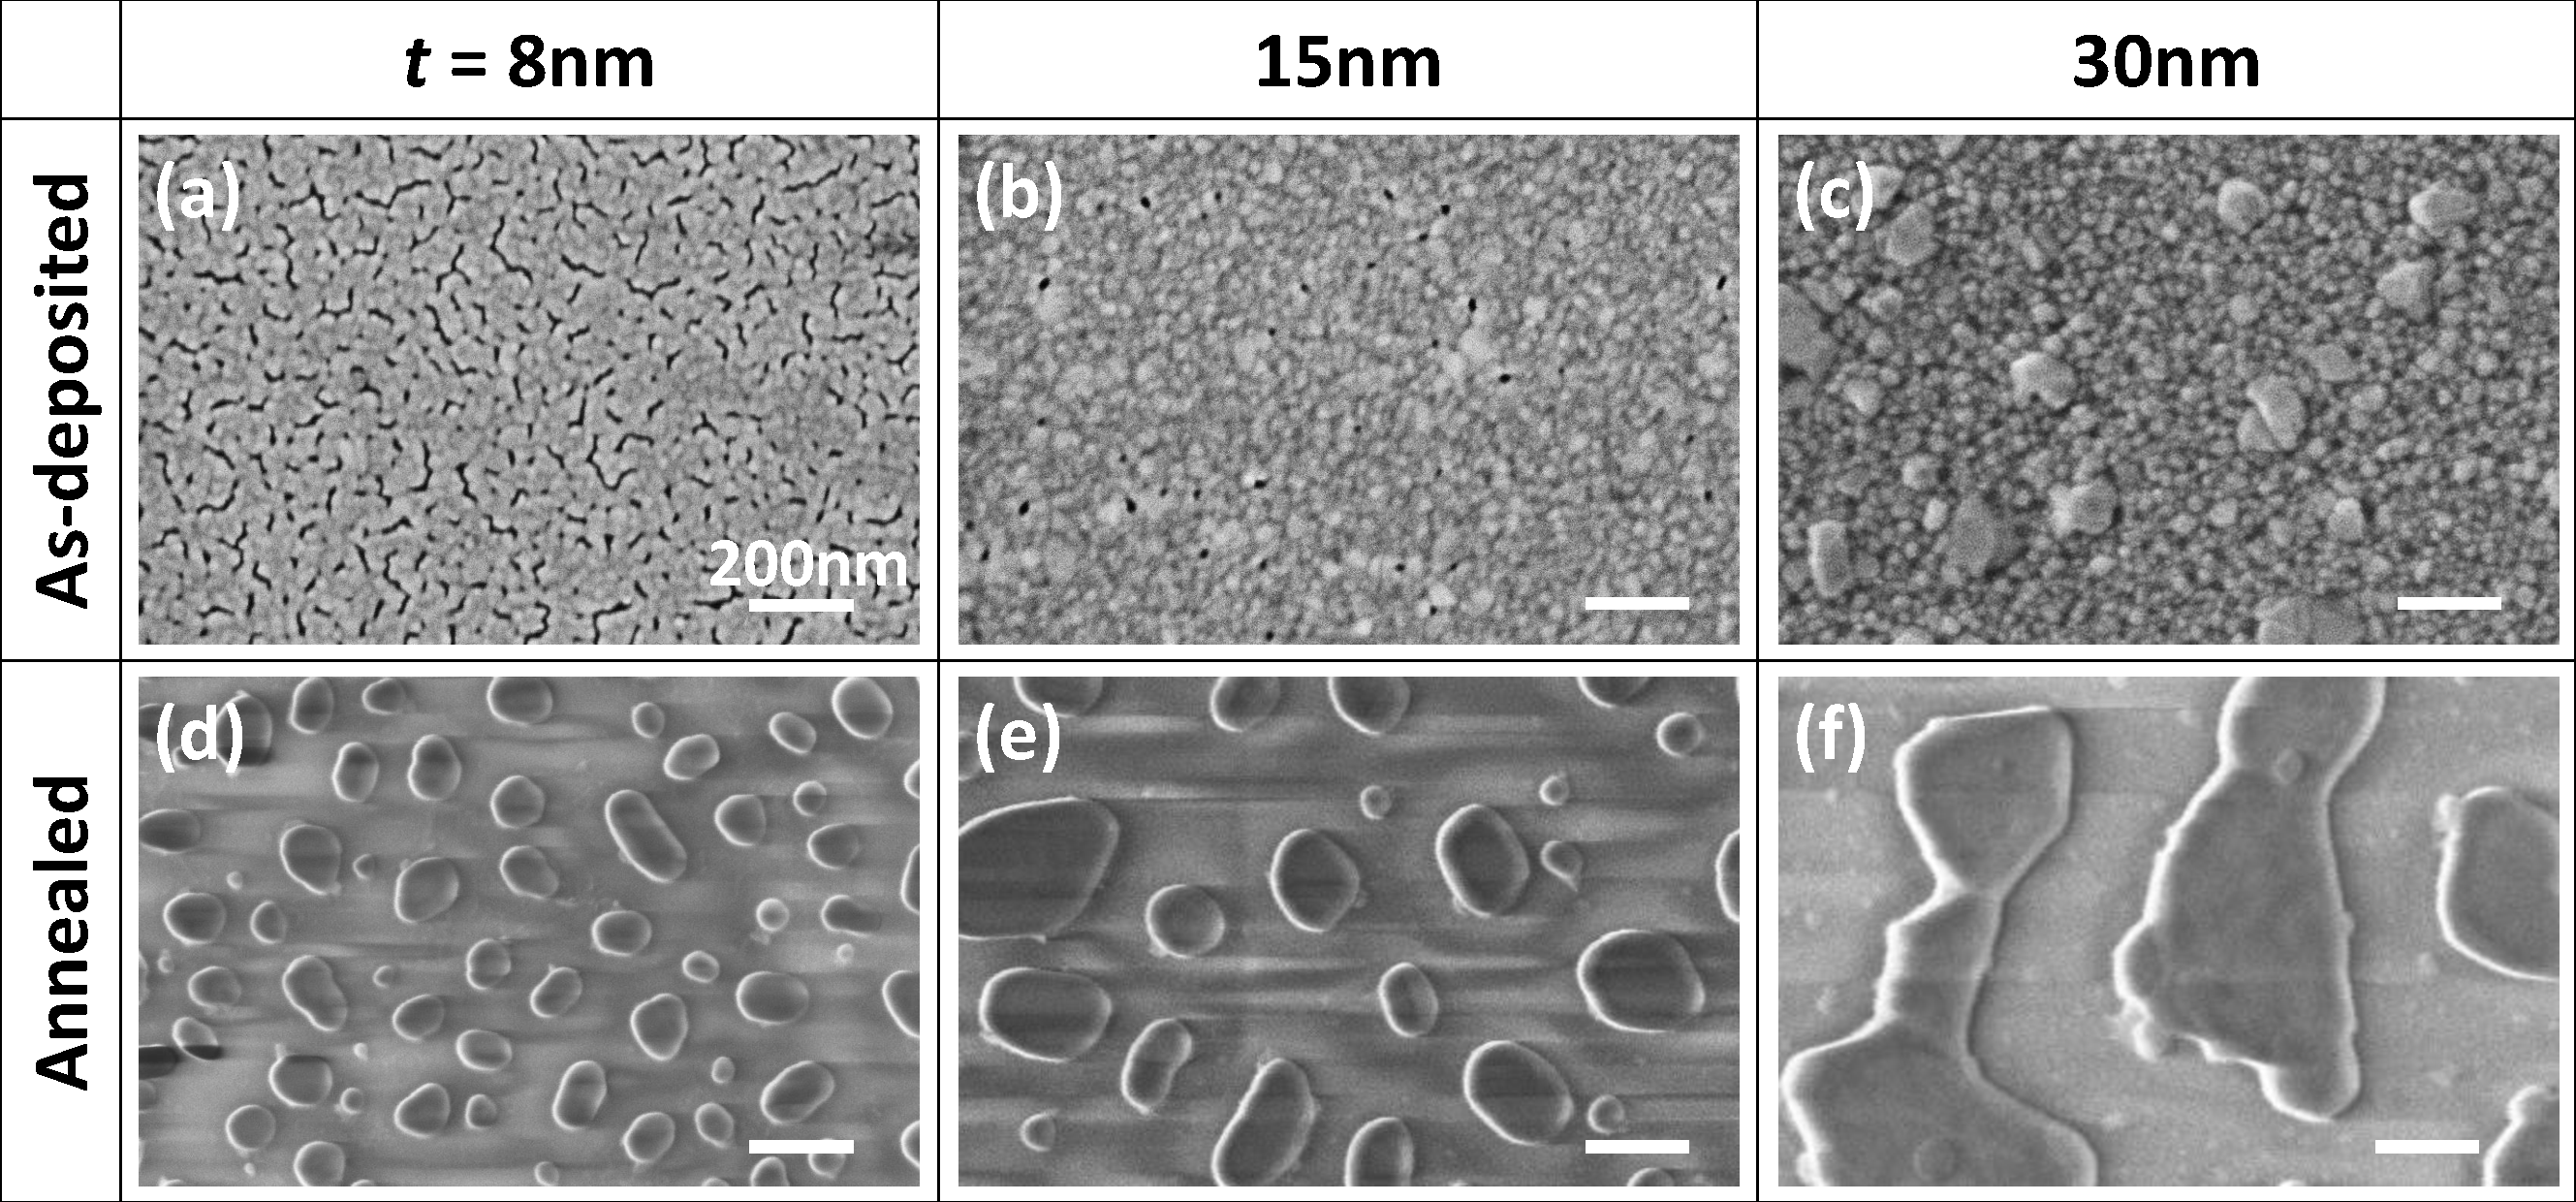
\includegraphics[width=\textwidth]{Fig1}
\caption{SEM images of (a-c) as-deposited and (d-f) annealed evaporated Au films. The initial deposited film thickness is labelled.}
\label{6Fig1}
\end{figure}
SEM images of evaporated Au films on glass shown the formation of a continuous film when 30\,nm is deposited [Fig.\,\ref{6Fig1}(c)], however the film is very rough and non-uniform. As the deposited thickness decreases [Figs.\,\ref{6Fig1}(a,b)] the films become smoother, however due to the weak Au-glass interaction dewetting is observed. As a result of annealing the Au atoms diffuse on the substrate and form distinct islands [Figs.\,\ref{6Fig1}(d-f)]. The islands become smaller in both lateral size and height [Fig.\,\ref{6Fig2}], and their shapes more uniformly ellipsoidal as $t$ decreases, and for 8\,nm we observe islands with size $50-100$\,nm, height $\sim$70\,nm, and separation $100-200$\,nm. The decrease in size can also be seen in 100$\times$ magnification DF images, where the scattering from the islands due to the LSP resonances become progressively is broadband and appears white for 30\,nm, but becomes progressively redder as the island size decreases [Fig.\,\ref{6Fig2}]. 
\begin{figure}[ht] 
\centering    
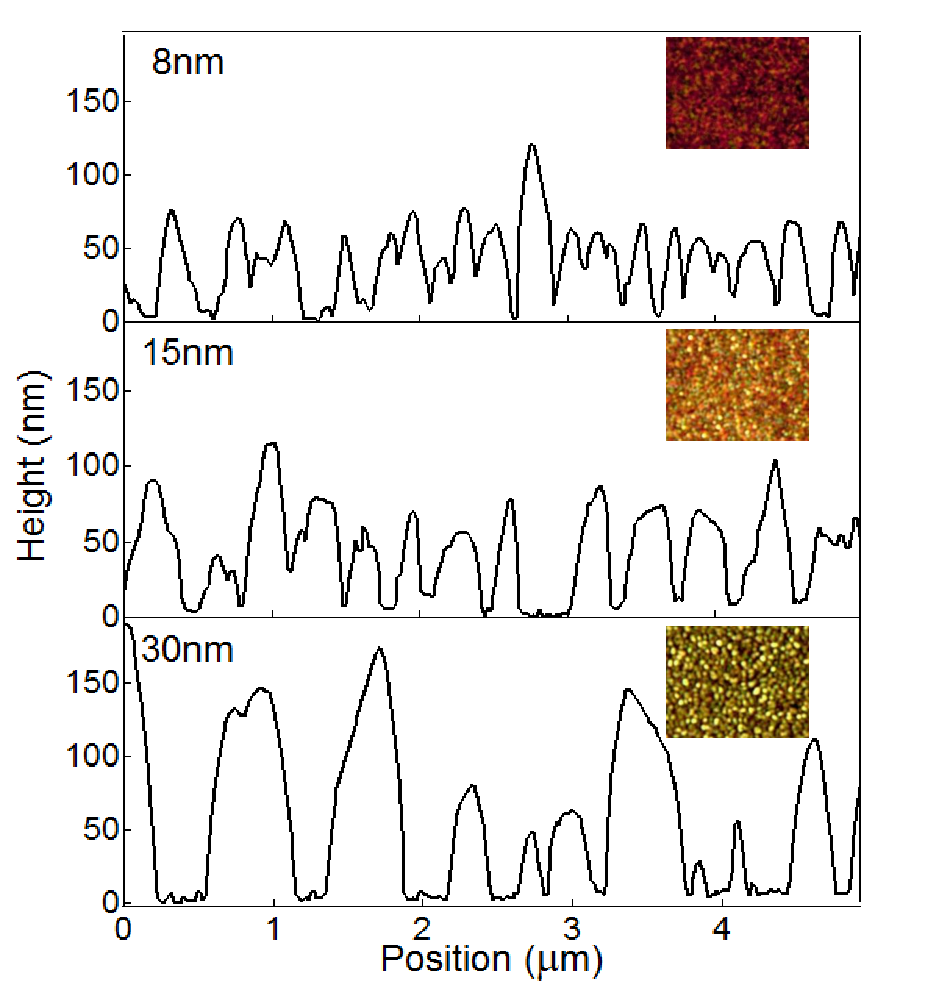
\includegraphics[width=0.8\textwidth]{Fig2}
\caption{AFM profiles of annealed Au metal island films. The deposited film thickness is labelled. Insets show 100$\times$ magnification DF images of the samples.}
\label{6Fig2}
\end{figure}
The change in the LSP resonance can be quantified optically using optical spectra. Fig.\,\ref{6Fig3} shows the extinction spectra for 8\,nm as-deposited and annealed Au films. We observe a resonance at 570\,nm in the extinction in the as-deposited film, however this is due to the roughness of the film and therefore has a large width of 245\,nm. In the annealed film we observe a resonance at 550\,nm with linewith 50\,nm due to the LSPs in the nano-islands, and using Mie theory this corresponds to a spherical particle with a diameter of 100\,nm.
\subsection{CHPI-coated Au metal island films}
\begin{figure}[ht] 
\centering    
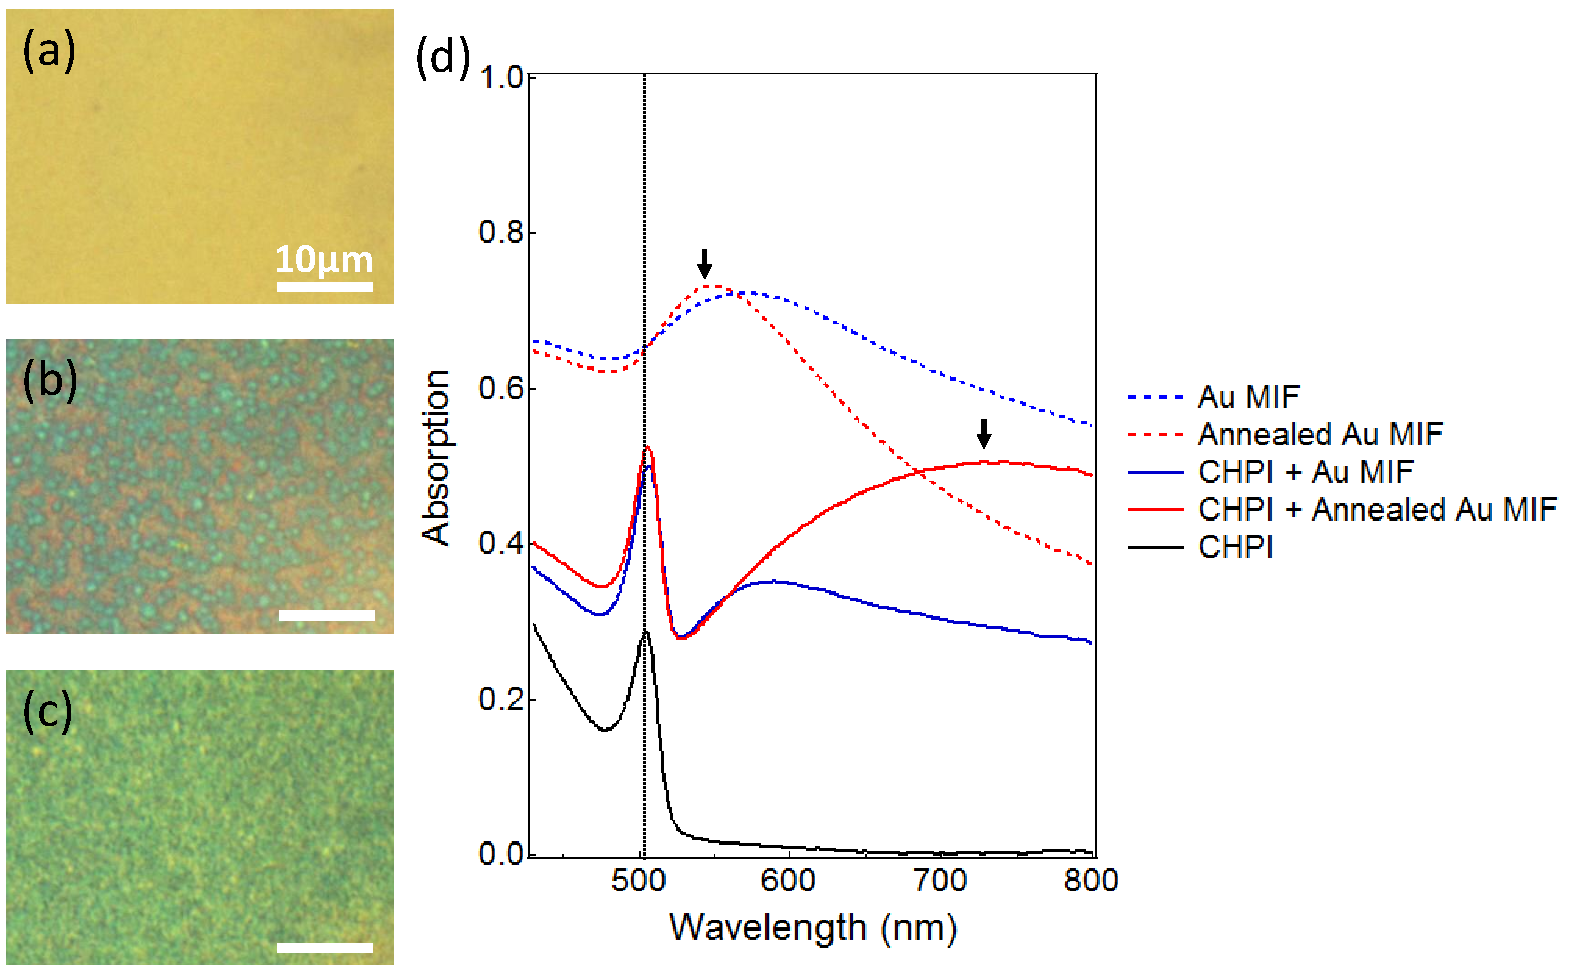
\includegraphics[width=\textwidth]{Fig3}
\caption{BF images at 100$\times$m magnification for CHPI films on (a) glass, (b) 8\,nm evaporated Au film, and (c) 8\,nm annealed Au metal island film. (d) Extinction spectra at 5$\times$ magnification. The exciton wavelength of the CHPI film is marked by the dashed line, and SPP resonances by arrows. The CHPI + (annealed) Au spectra are offset for clarity.}
\label{6Fig3}
\end{figure}
BF images at 100$\times$ magnification show the formation of CHPI on $t$=8\,nm Au samples (green areas in Figs.\,\ref{6Fig3}(b,c)), however the CHPI film is much rougher than on glass [Fig.\,\ref{6Fig3}(a)], and some dewetting can be seen. The exciton resonance at 505\,nm is observed for all three films, confirming the formation of the correct MQW structure. We observe a redshift in the LSP resonance of the Au nano-islands for annealed films due to the CHPI: the resonance changes from 550\,nm to 735\,nm, with a considerable increase in the linewidth due to the non-uniform CHPI coating. The redshift predicted by Mie theory for a spherical particle embedded in a medium with the refractive index of CHPI is 625\,nm, and the discrepancy may be due to the ellipsoidal shape of the Au islands in the MIF. Note however that excitons in CHPI are completely unaffected by the Au films, keeping the same wavelength and linewidth, although the overall magnitude of the extinction has increased due to the Au films.
%CHPI+annealed Au LSP linewidth ~500nm+?

\subsection{Ag metal island films}
\begin{figure}[ht] 
\centering    
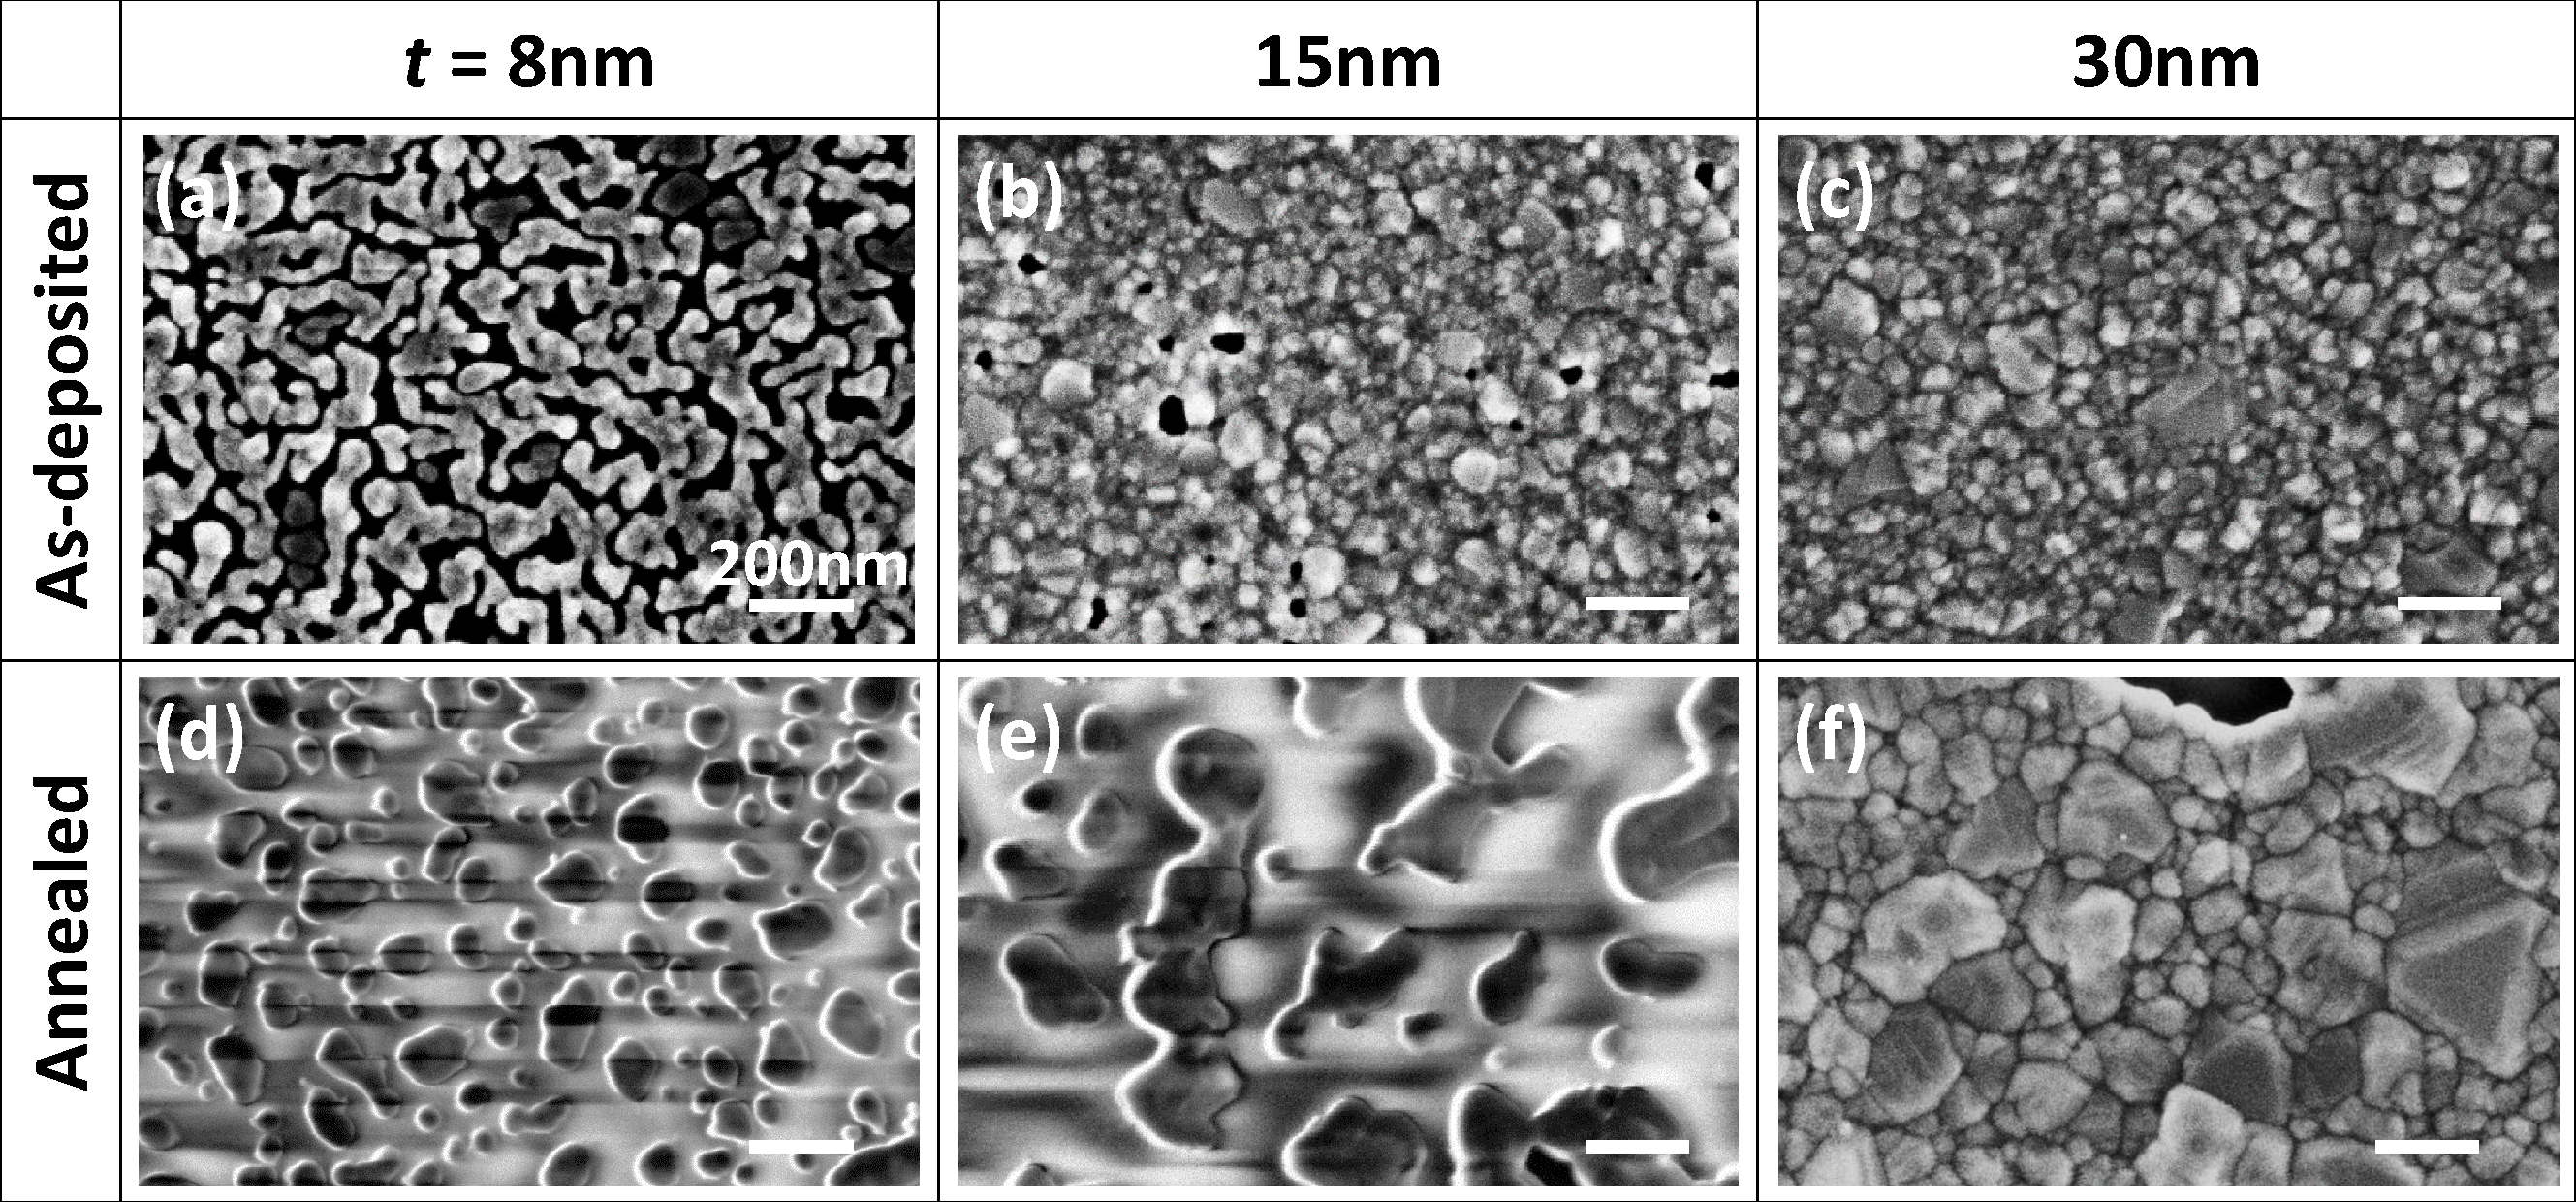
\includegraphics[width=\textwidth]{Fig4}
\caption{SEM images of (a-c) as-deposited and (d-f) annealed evaporated Ag films. The initial deposited film thickness is labelled. Dark areas/streaks are seen in (a, d, e) due to charging of the sample.}
\label{6Fig4}
\end{figure}
The morphology of Ag evaporated films glass show similar trends to Au films: rough films lead to smoother dewetted films with decreasing $t$, and the formation of MIFs when the as-deposited films are annealed [Fig.\,\ref{6Fig4}]. However the interactions between Ag atoms and glass is clearly strongly than with Au, as for 30\,nm films annealing only causes coalescence and larger grains, not well separated islands. Annealed 8,\nm Ag MIFs consist of ellipsoidal islands with lateral size $40-100$\,nm, height $\sim80$\,nm, and separation $50-150$\,nm. DF images [Fig.\,\ref{6Fig5}] also show broadband white scattering for larger islands. 

\begin{figure}[ht] 
\centering    
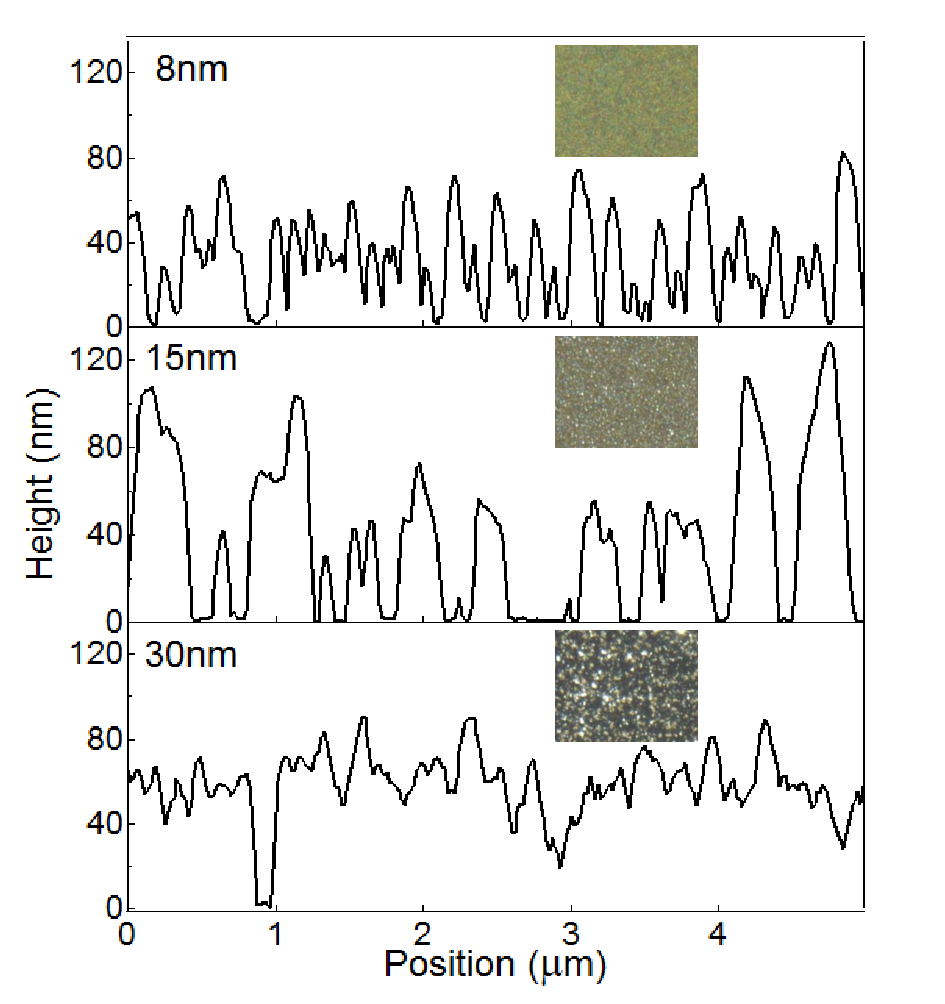
\includegraphics[width=0.8\textwidth]{Fig5}
\caption{AFM profiles of annealed Ag metal island films. The deposited film thickness is labelled. Insets show 100$\times$ magnification DF images of the samples.}
\label{6Fig5}
\end{figure}

As seen in the SEM images, for $t>8$\,nm as-deposited Ag films are essentially continuous with some dewetting, and the extinction spectra are similar to that of a bulk Ag film, with low extinction at visible wavelengths, increasing extinction up to the band gap $\sim300$\,nm [Fig\,\ref{6Fig6}(a)]. However resonances can be observed for lower $t$ films, particular for 2\,nm as-deposited films with a resonance at 560\,nm and linewidth 175\,nm, suggesting the formation of islands even without annealing (see below). 

After annealing, the LSP resonance of the Ag islands dominated the extinction spectra [Fig.\,\ref{6Fig6}(b)]. Comparing the extinction peaks [Fig.\,\ref{6Fig6}(c)], we see that the positions of the extinction peaks do not change significantly with $t$, however there is a clear decrease in the linewidth of the $t$=2\,nm film compared to the others. The relative stability of the LSP resonance position suggests that the average island size does not change with $t$, however for larger $t$ we may have a larger deviation in the shape and sizes of the islands, leading to a superposition of many resonance wavelengths and higher order LSP modes. The resonance wavelength of $\sim$440\,nm for the Ag islands is larger than the predicted value of an 100\,nm spherical particle from Mie theory (380\,nm), which may be due to both the ellipsoidal nature of the Ag islands, as well a potential oxidation layer formed on the surface of the islands. 
\begin{figure}[ht] 
\centering    
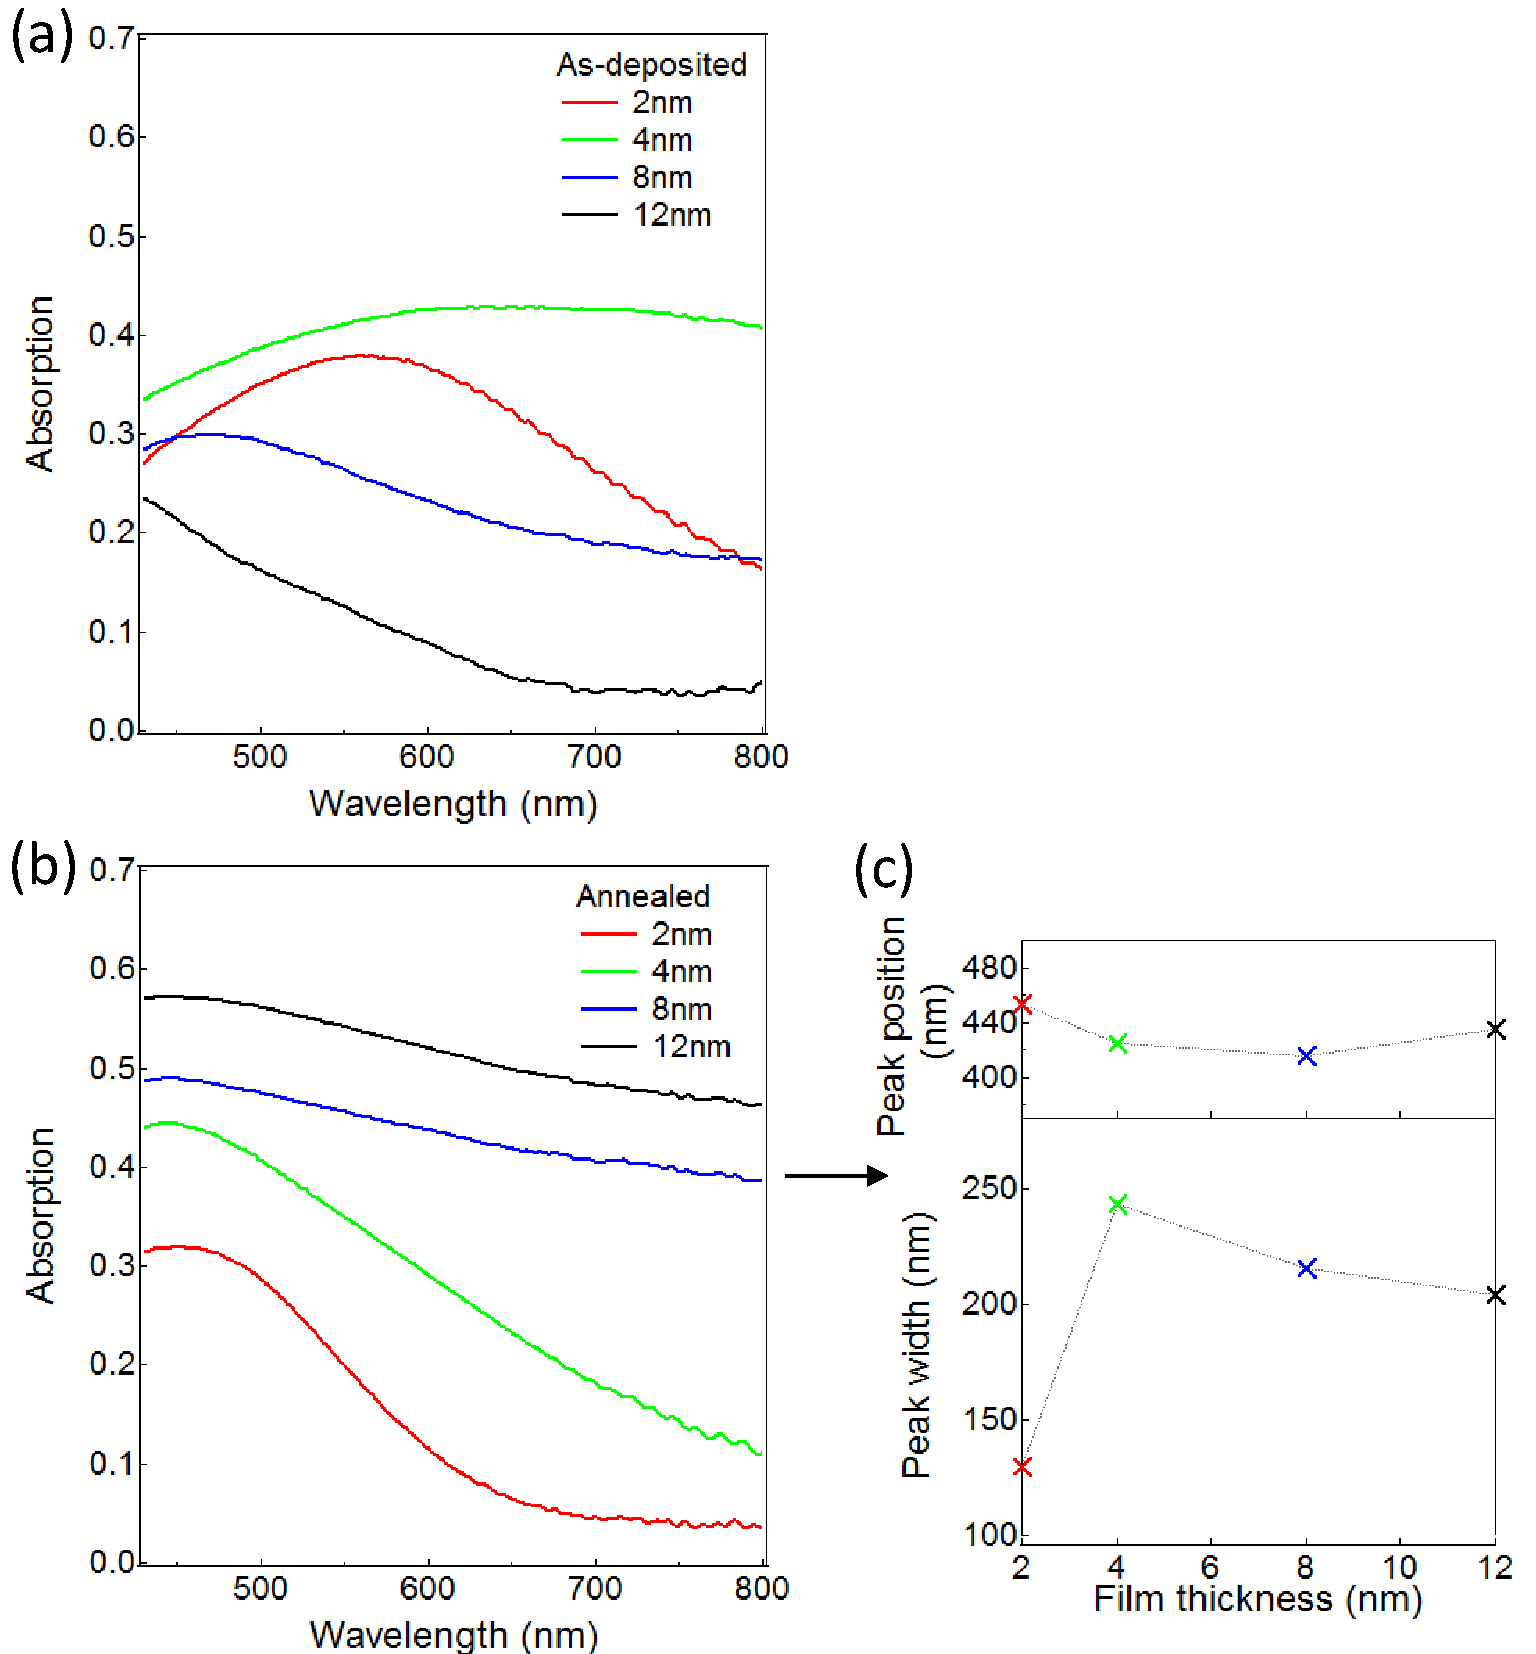
\includegraphics[width=\textwidth]{Fig6}
\caption{Extinction spectra collected at 5$\times$ magnification for (a) as-deposited Ag films and (b) annealed Ag metal island films with the labelled thickness. (c) Extinction peak position and linewidth for the spectra in (b).}
\label{6Fig6}
\end{figure}

\subsection{CHPI-coated Ag metal island films}
\begin{figure}[ht] 
\centering    
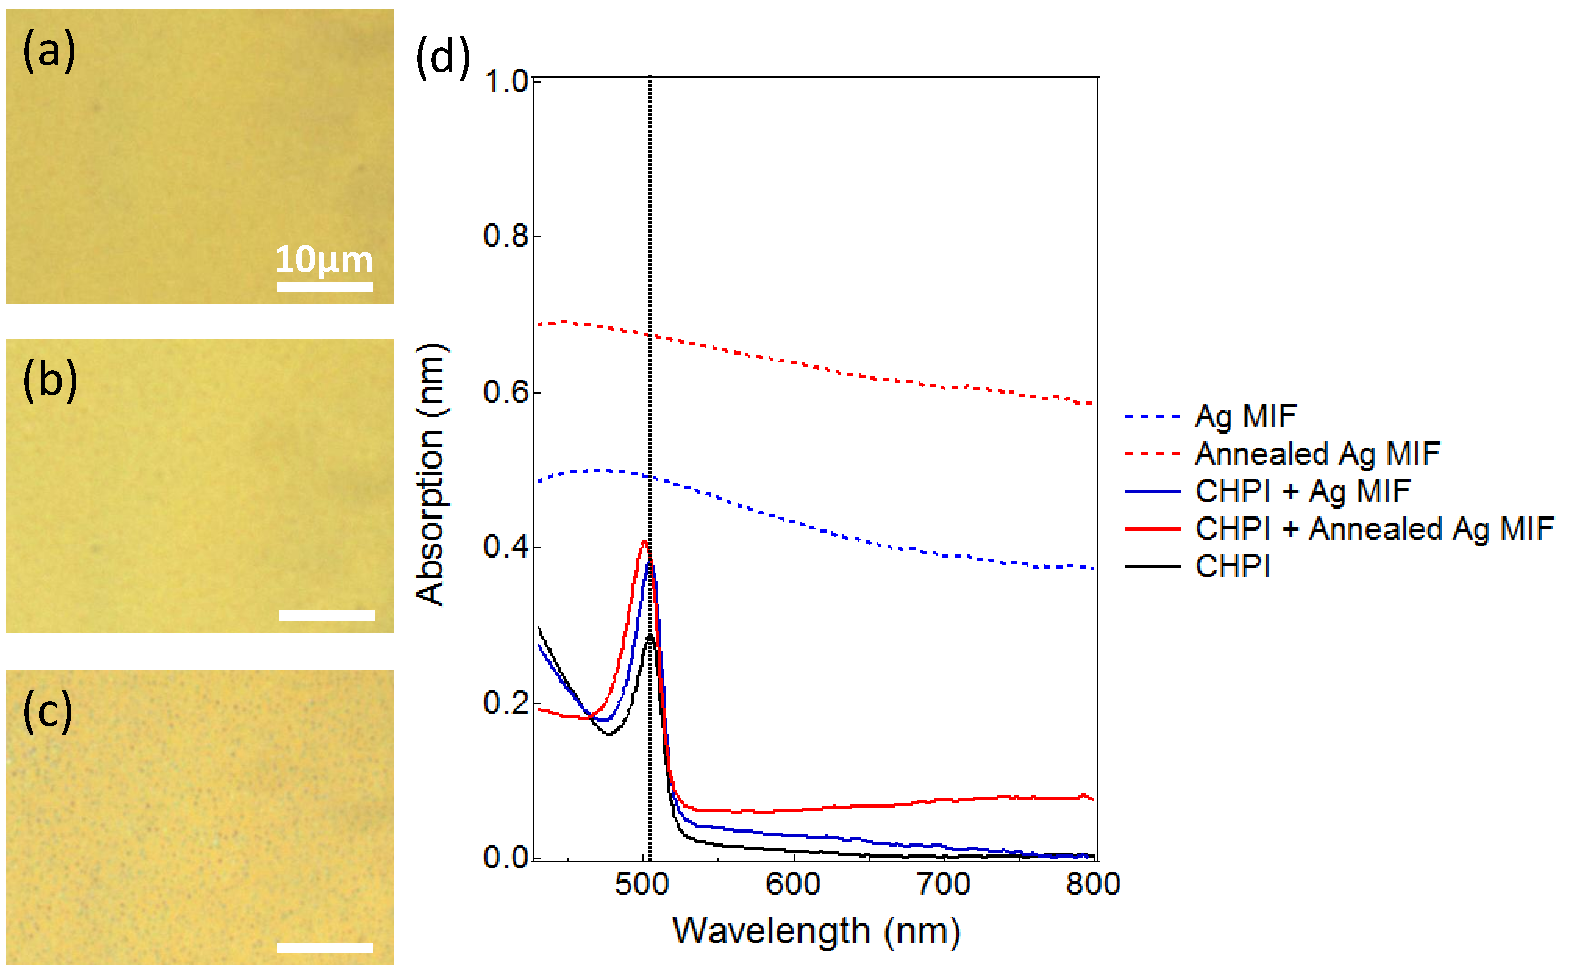
\includegraphics[width=\textwidth]{Fig7}
\caption{BF images at 100$\times$m magnification for CHPI films on (a) glass, (b) 8\,nm evaporated Ag film, and (c) 8\,nm annealed Ag metal island film. (d) Extinction spectra at 5$\times$ magnification. The exciton wavelength of the CHPI film is marked by the dashed line. The (annealed) Ag spectra are offset for clarity.}
\label{6Fig7}
\end{figure}
CHPI coated Ag films behave similarly for all $t$, so here we use $t$=8\,nm as an example. BF images at 100$\times$ magnification show CHPI films deposited on as-deposited and annealed Ag films appear very similar to CHPI films deposited on glass [Fig.\,\ref{6Fig7}(a-c)], although some non-uniformity is observed in the case of annealed Ag MIF. The extinction spectra of CHPI coated as-deposited Ag film is very similar to the spectra of CHPI film on glass (exciton at 505\,nm). However the Ag islands of the annealed film causes a blueshift of the exciton wavelength to 500\,nm, we see no appearance of the island LSP resonance, and there is an overall increase in the exciton extinction peak as a result of the Ag islands. Together this indicates weak coupling between the Ag LSP and excitons and enhancement in exciton absorption due to the near-field of the LSP. 

\subsection{Ag islands on CHPI films}
\begin{figure}[ht] 
\centering    
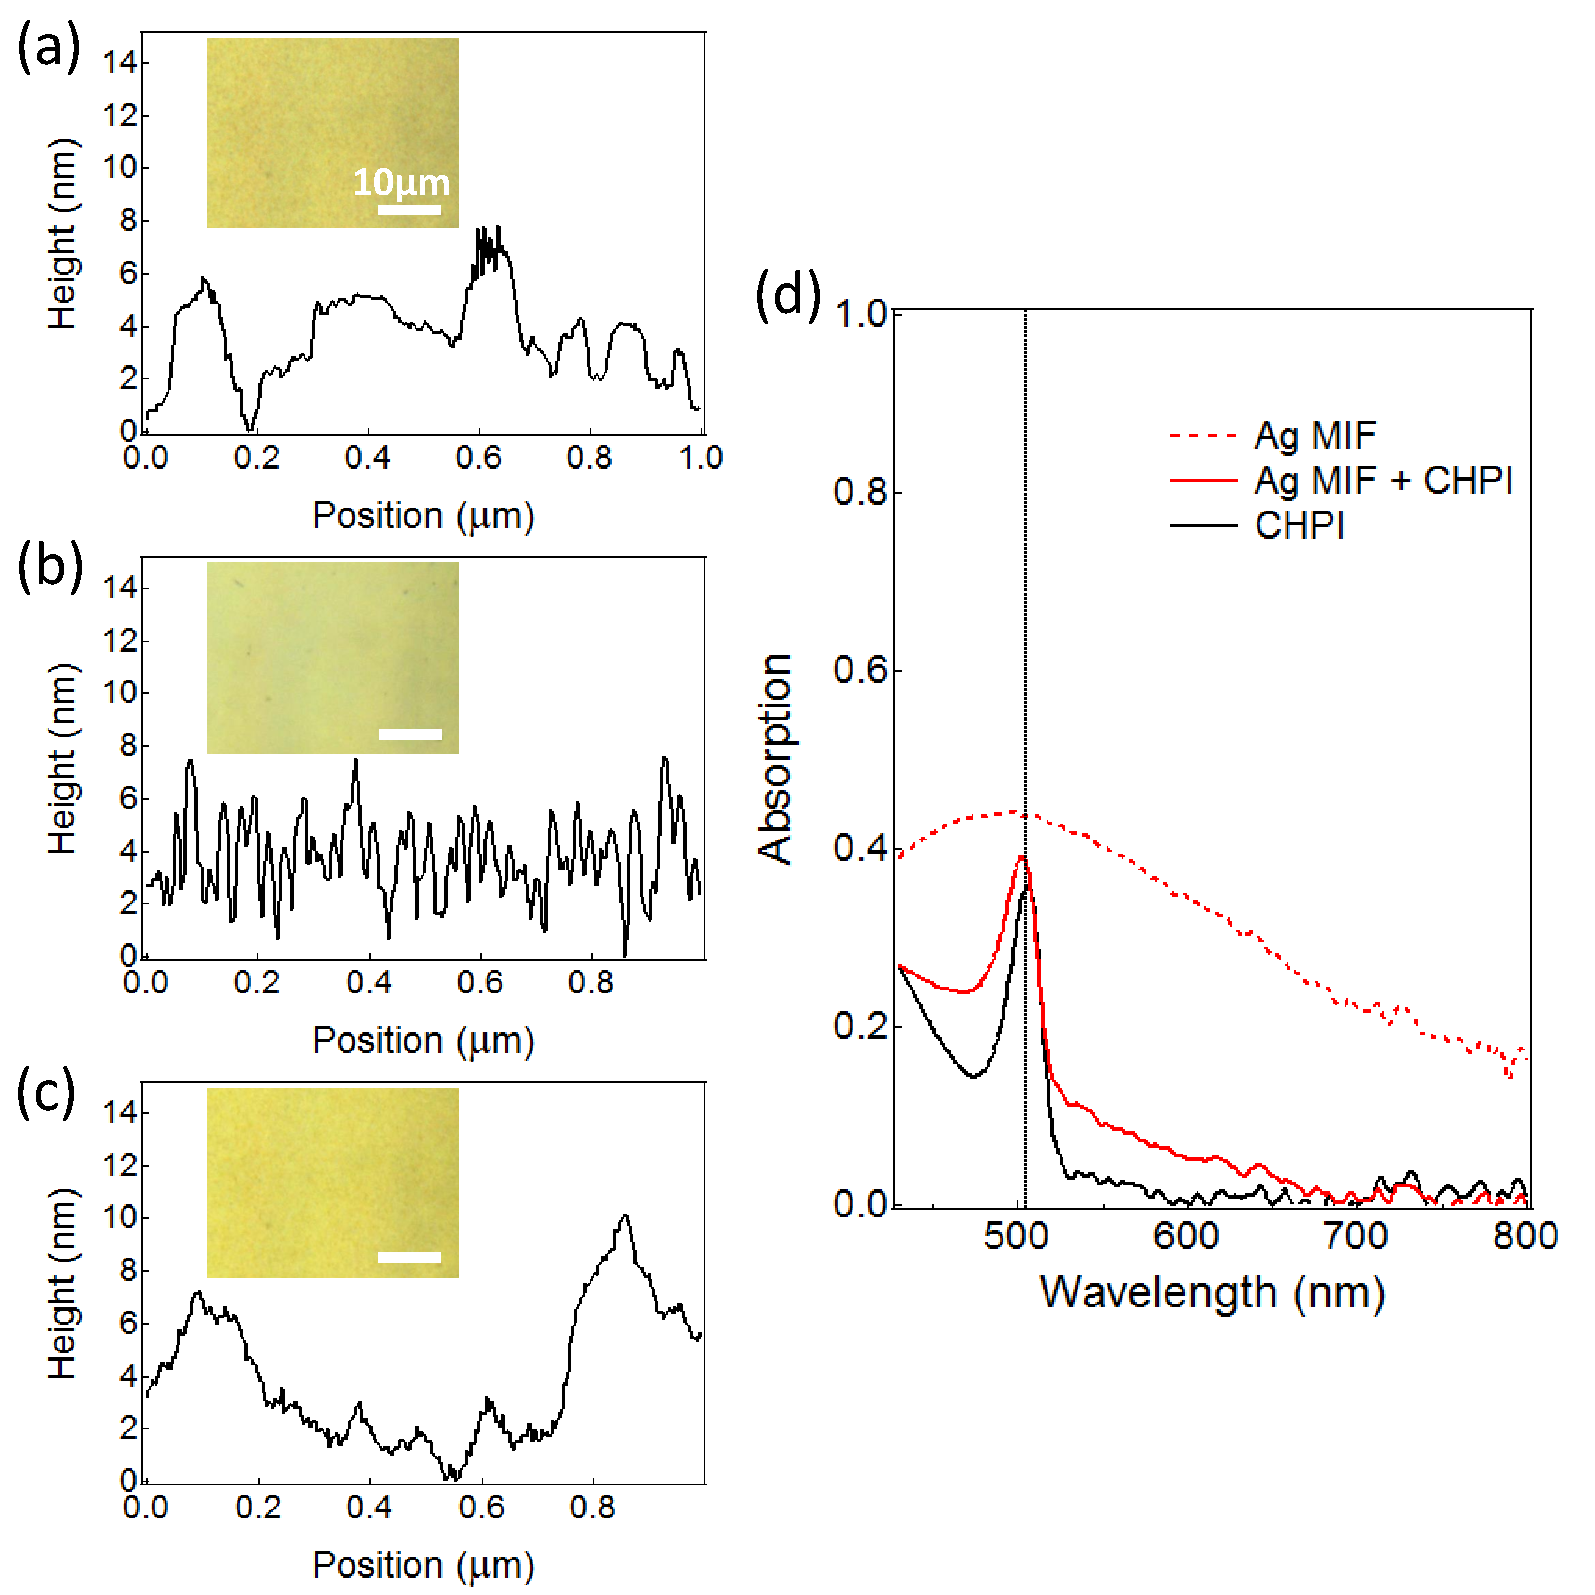
\includegraphics[width=\textwidth]{Fig8}
\caption{AFM profiles of (a) CHPI film on glass, (b) 2\,nm evaporated Ag film on glass, and (c) 2\,nm evaporated Ag film on CHPI. The insets show 100$\times$ magnification BF images of the samples. (d) Extinction spectra at 5$\times$ magnification. The exciton wavelength of the CHPI film is marked by the dashed line. The Ag spectrum is offset for clarity.}
\label{6Fig8}
\end{figure}
Instead of coating Ag MIF films with CHPI, we also fabricated samples of Ag islands on top of a CHPI film on glass. Since the organic molecules undergo a melting transition $\sim$80$^{\circ}$C \cite{Barman2003}, we thermally evaporate only 2\,nm of Ag to prevent any degradation of the CHPI film due to heat. The AFM profile of a 2\,nm as-deposited Ag film on glass [Fig.\,\ref{6Fig8}(b)] shows the formation of separated metal islands, with lateral size $\sim$30\,nm and height $\sim$6\,nm. The AFM profile of a Ag MIF on CHPI is dominated by the surface roughness of the CHPI film ($\sim$5\,nm, \textit{cf} Fig.\,\ref{6Fig8}(a)), however some high frequency noise on the order of the island sizes can also be seen. However the island features are not distinct from the CHPI film, which suggests the particles may be embedded in the CHPI film. Looking at the extinction spectra [Fig.\,\ref{6Fig8}(d)], the strong exciton peak indicates that the MQW structure remains despite the thermal evaporation of Ag, and the interactions between the LSP of the Ag islands and the excitons leads to weak coupling, with a blueshift in the exciton wavelength of 4\,nm, similar to what was observed in the CHPI-coated Ag islands [Fig.\,\ref{6Fig7}(d)].

\section{Nanosphere lithography}
Nanosphere lithography involves the use of closely-packed 2D arrays of nano-/microparticles as lithography masks. Evaporation of metal through the mask followed by removal of the spheres leaves behind an array of metal islands on the substrate \cite{Haynes2001}. The geometry of the island array depends on the diameter of spheres $D$ used in the mask. For a colloidal monolayer, the island diameter is $0.223$, while the inter-island separation is $0.58D$ \cite{Hulteen1995}. The islands formed are triangular in shape due to the interstices between spheres, however for small $D$ the islands can become more spherical \cite{Hulteen1999}. Array geometry can also be controlled by changing the evaporation angle \cite{Haynes2002}.

Much like MIFs, the metallic islands produce a LSP peak in optical spectra, where the resonance wavelength depends on the size and shape of islands, as well as the dielectric environment \cite{Jensen2000}, and as such can be modelled as an array of dipoles \cite{Malinsky2001, Jensen1999}. However nanosphere lithography provides better control of the island geometry due to the periodicity of the microsphere mask, so should provide a sharper LSP resonance when compared with MIFs.

\subsection{Experimental methods}
We use 460\,nm diameter polystyrene (PS) microspheres from Sigma Aldrich to create the colloidal monolayer. The 10\% microsphere solution is then diluted in a 1:1 miz with absolute ethanol. Glass substrates are cleaned as described in Sec.\,\ref{sec:glass} then plasma etched for 1\,minute to create a hydrophilic surface. The substrates are placed at a $10^{\circ}$ angle before a deionised water droplet is applied to cover the glass surface. A 2wt\% solution of sodium dodecylsulphate in water ($<0.5\,\mu$l) is then applied to the water surface, where the amphiphilic surface molecules acts to reduce the surface charges on PS microspheres. A pipette is used to spread the PS microsphere onto the droplet surface [Fig.\,\ref{6Fig9}(a)], and the water allowed to evaporate under standard conditions. 50\,nm of Au is then deposited on the samples using an electron-beam evaporator system under a pressure $\sim5\times10^{-6}$\,Torr at a rate of 1\AA/s. The PS microspheres are dissolved by placing the sample in a solution of dichloromethane for 30\,minutes, then sonicating the solution for 5\,minutes. CHPI-coating is then produced by spin coating a CHPI/THF solution onto the island samples under a dehydrated atmosphere. Optical characterisation is performed by taking 400 scans over a $50\times50\,\mu$m$^{2}$ region, then averaged to produce the spectra shown. 

\subsection{Au islands}
Closely-packed 2D arrays of PS microspheres are formed using this technique [Fig.\,\ref{6Fig9}(b)], and the ordering is best at contact lines due to the coffee ring effect. After removal of PS, triangular islands are left behind on the glass substrate [Fig.\,\ref{6Fig9}(c)] with lateral size $\sim$90\,nm. We can see from Fig.\,\ref{6Fig9}(c) that even in the best areas we do not uniformly find well-separated triangular islands. Due to small deviations in the microsphere packing bow-tie shaped islands can form, or lines of Au in a gap between domains. However in the extinction spectra of such island samples [Fig.\,\ref{6Fig10}] we do observe an LSP resonance at 590\,nm with a linewidth of 80\,nm.
\begin{figure}[ht] 
\centering    
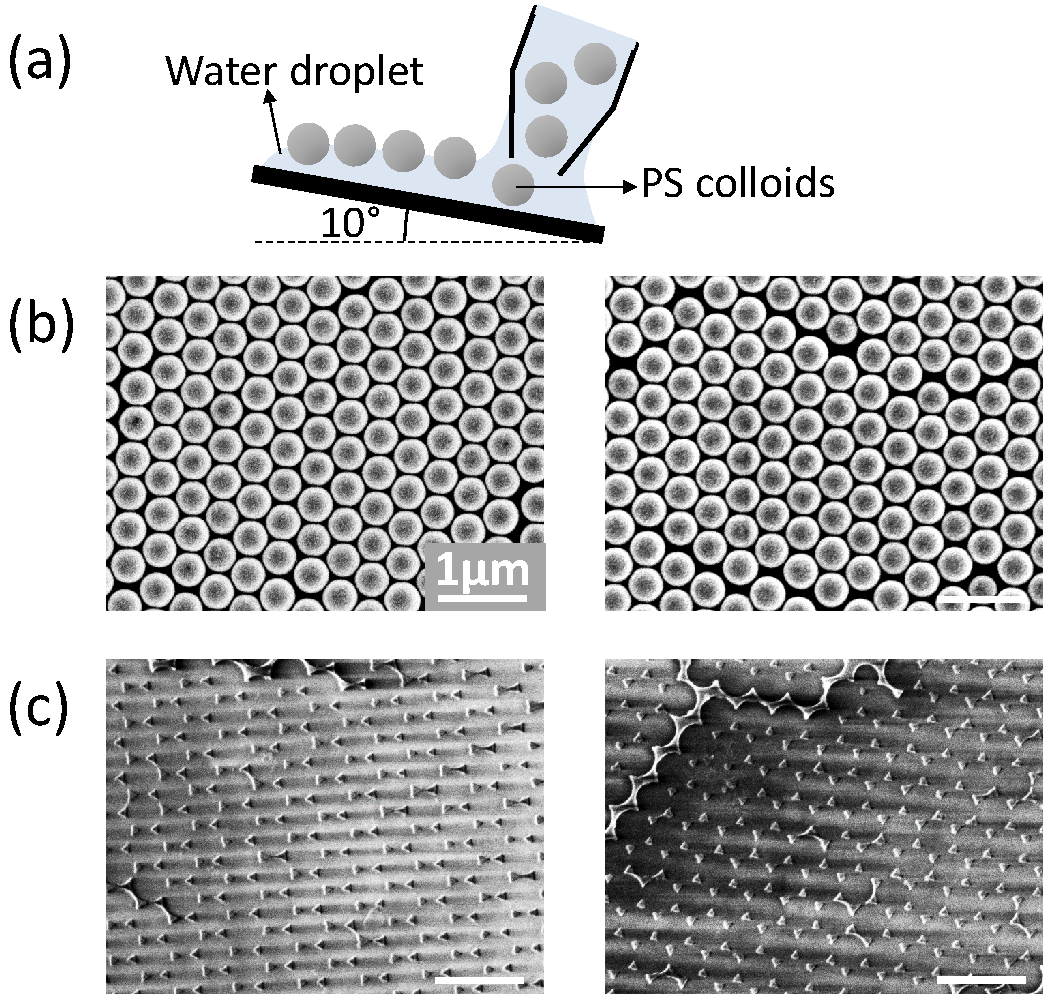
\includegraphics[width=0.8\textwidth]{Fig9}
\caption{(a) Schematic illustration of the transfer of 460\,nm PS colloids to a water droplet via a pipette. (b) SEMs of colloid monolayer formed after the water droplet evaporates under standard conditions. (c) SEMs of triangular islands formed after evaporation of Au onto colloid monolayers and dissolving the PS.}
\label{6Fig9}
\end{figure}

\subsection{CHPI-coated Au islands}
Similar to the CHPI-coated Au MIF, strong exciton peaks in the extinction spectra of CHPI-coated Au islands indicate formation of the correct MWQ structure. The exciton wavelength is unaffected by the Au and remains at 505\,nm. As before, the LSP resonance redshifts due to the CHPI coating, and the linewidth broadens to $\sim$150\,nm. We observe a systematic increase of the LSP redshift as a result of increasing spin speed, and attribute this to more complete CHPI encapsulation of the Au islands due to larger forces induced by the higher spin speeds.
\begin{figure}[ht] 
\centering    
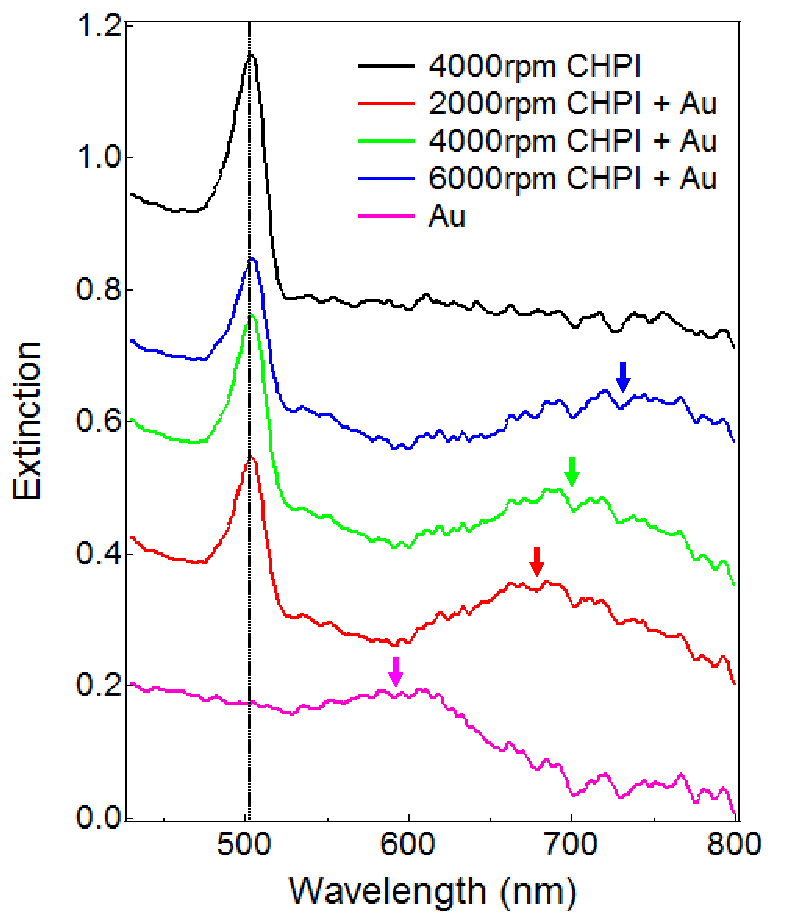
\includegraphics[width=0.8\textwidth]{Fig10}
\caption{Extinction spectra for CHPI-coated Au islands as labelled. Arrows indicate the positions of LSP resonances, and a dashed line indicates the exciton wavelength.}
\label{6Fig10}
\end{figure}

\section{Conclusions}
Evaporation of noble metals can be use to create ellipsoidal nanoparticles on a glass substrate due to poor adhesion of the metal atoms. Optically the electrons in such particles can oscillate in phase to create LSP resonances. The resonance wavelength can be tuned using the shape and size of the particles, and can be changed by changing the dielectric environment around the particles. When the LSP resonance is far off-resonance with excitons, as is the case with Au, the perovskite thin film merely acts as a high refractive index medium and causes a redshift in the LSP wavelength. However is the two resonances are closer together in energy, as with Ag islands, weak coupling can occur, causing a blueshift in the exciton wavelength by 5\,nm, and enhancing the exciton absorption due to the enhanced electric field of the LSP. Such absorption enhancement has been investigated and is of particular interest for the design of solar cells \cite{Alemu2014, Zheng2011, Xu2013, Spinelli2012}.

In order to observe strong coupling between LSPs and excitons, one problem may be with the width of the LSP resonance. The large variation in shape and size of metal particles in MIFs could potentially be an issue. However from our experiments the controllable islands created using nanosphere lithography do not create a marked improvement in the optical signature of the LSP resonance. A potential future exploration could be to use chemically created metallic NPs, which are often pre-screened for size. However a method of controllable assembling a dense array of individual NPs from solution will need to be explored.